% READ-Grid: Run 1 -> Run 2 pipeline repair map
% Compile: pdflatex fig_readgrid_pipeline.tex
\documentclass[border=6pt]{standalone}
\usepackage[T1]{fontenc}
\usepackage{lmodern}
\usepackage{amsmath}
\usepackage{tikz}
\usetikzlibrary{arrows.meta,calc,positioning}

\definecolor{ink}{RGB}{38,42,48}
\definecolor{deffill}{RGB}{252,240,238}
\definecolor{defline}{RGB}{168,60,50}
\definecolor{fixfill}{RGB}{236,242,236}
\definecolor{fixline}{RGB}{78,112,86}

\tikzset{
  stage/.style 2 args={rectangle, draw=#1, fill=#2, line width=0.6pt,
    align=center, text=ink, text width=3.85cm, minimum height=2.0cm,
    inner sep=3pt, outer sep=0pt,
    execute at begin node={\hyphenpenalty=10000\relax}},
  repair/.style={-{Stealth[length=2.2mm,width=1.6mm]}, line width=0.8pt,
    draw=ink!55},
}

\begin{document}
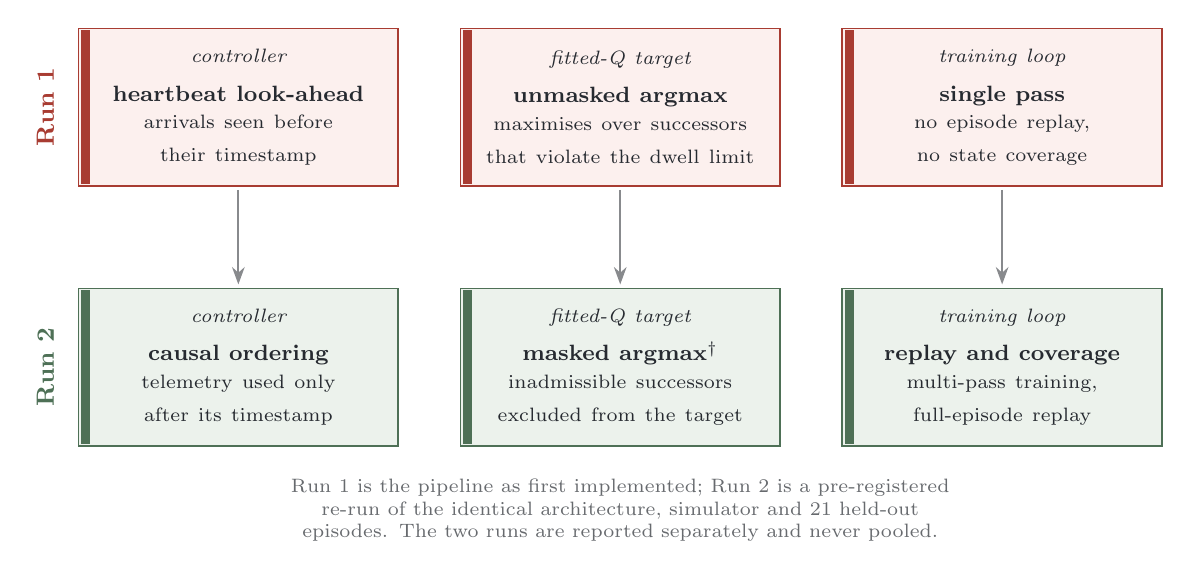
\begin{tikzpicture}[x=1cm, y=1cm, line width=0.6pt, color=ink]

% ---------------- row tags ----------------
\node[rotate=90, font=\small\bfseries, text=defline] at (0.55,7.60) {Run 1};
\node[rotate=90, font=\small\bfseries, text=fixline] at (0.55,4.30) {Run 2};

% ---------------- Run 1 ----------------
\node[stage={defline}{deffill}] (a1) at (3.00,7.60)
  {{\scriptsize\itshape controller}\\[2pt]
   {\footnotesize\bfseries heartbeat look-ahead}\\[2pt]
   {\scriptsize arrivals seen before\\their timestamp}};

\node[stage={defline}{deffill}] (a2) at (7.85,7.60)
  {{\scriptsize\itshape fitted-Q target}\\[2pt]
   {\footnotesize\bfseries unmasked argmax}\\[2pt]
   {\scriptsize maximises over successors\\that violate the dwell limit}};

\node[stage={defline}{deffill}] (a3) at (12.70,7.60)
  {{\scriptsize\itshape training loop}\\[2pt]
   {\footnotesize\bfseries single pass}\\[2pt]
   {\scriptsize no episode replay,\\no state coverage}};

% ---------------- Run 2 ----------------
\node[stage={fixline}{fixfill}] (b1) at (3.00,4.30)
  {{\scriptsize\itshape controller}\\[2pt]
   {\footnotesize\bfseries causal ordering}\\[2pt]
   {\scriptsize telemetry used only\\after its timestamp}};

\node[stage={fixline}{fixfill}] (b2) at (7.85,4.30)
  {{\scriptsize\itshape fitted-Q target}\\[2pt]
   {\footnotesize\bfseries masked argmax$^{\dagger}$}\\[2pt]
   {\scriptsize inadmissible successors\\excluded from the target}};

\node[stage={fixline}{fixfill}] (b3) at (12.70,4.30)
  {{\scriptsize\itshape training loop}\\[2pt]
   {\footnotesize\bfseries replay and coverage}\\[2pt]
   {\scriptsize multi-pass training,\\full-episode replay}};

% ---------------- left colour rules ----------------
\foreach \x in {0.97,5.82,10.67}{
  \fill[defline] (\x+0.03,6.62) rectangle (\x+0.15,8.58);
  \fill[fixline] (\x+0.03,3.32) rectangle (\x+0.15,5.28);
}

% ---------------- repair arrows ----------------
\foreach \c in {3.00,7.85,12.70}{
  \draw[repair] (\c,6.55) -- (\c,5.35);
}

% ---------------- note ----------------
\node[anchor=north, font=\scriptsize, text=ink!70, align=center,
      text width=12.6cm, execute at begin node={\hyphenpenalty=10000\relax}]
  at (7.85,3.00)
  {Run 1 is the pipeline as first implemented; Run 2 is a pre-registered re-run
   of the identical architecture, simulator and 21 held-out episodes. The two
   runs are reported separately and never pooled.};

\end{tikzpicture}
\end{document}
